\chapter{Experiments}
\label{expchap}
In order to test the effectiveness of the network, we train both an LLM model and an LSTM model on several different datasets. We both developed synthetic datasets, and natural datasets found from various different sources.
\section{Datasets}
\subsection{Synthetic Datasets}
The synthetic datasets discussed below were created to attempt to mimic potential tasks that the network will face in natural datasets. These datasets were adapted from tasks introduced in Discrete-Event Continuous-Time Recurrent Nets \cite{DECTRN}.
\subsubsection{Accumulator}
The accumulator dataset has sequences of events generated via Poisson processes. Each poisson process has a randomly generated rate, and events are labelled by which process they are generated by. When an event is generated, an associated accumulator is incremented by a set amount. Over time, the accumulators for each label are exponentially decayed. At the end of the sequence, the sequence is labelled by the strongest accumulator. An example from this dataset can be seen in Figure \ref{fig:accum} with the accumulator function included. 
\begin{figure}
    \centering
    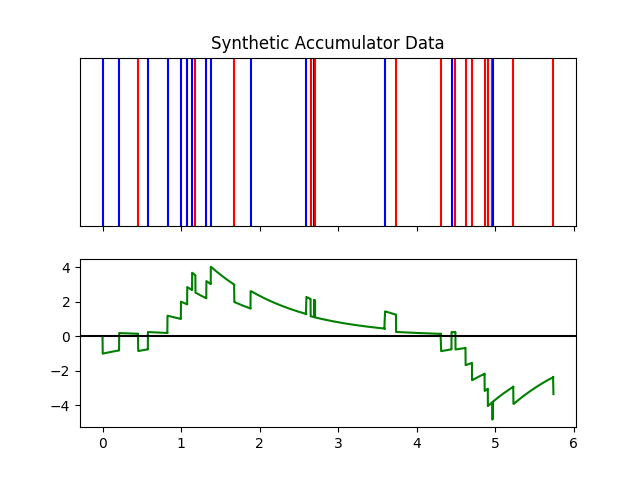
\includegraphics{figures/accum1.png}
    \caption{Accumulator}
    \label{fig:accum}
    Visualization of the a two event type accumulator sequence, and the associated classifier function over time.
\end{figure}
\subsubsection{Rhythm}
\label{sec:rhythm}
The Rhythm dataset contains events followed by a set lag. Each event label corresponds to a lag time (i.e. 1, 2, 4, 8...) between that event and when the next will occur. Each event is chosen uniformly from the different event types. The task itself is presented as a classification, where a sequence is labelled with a 1 if the sequence is generated with the normal lag times, or a 2 is the sequence is generated with altered lag times. This can be thought of as similar to anomaly detection, where an ideal classifier would identify the sequence as 1 up until it ``sees" a changed lag time. There is an example sequence from this dataset in Figure \ref{fig:rhythm}.
\begin{figure}
    \centering
    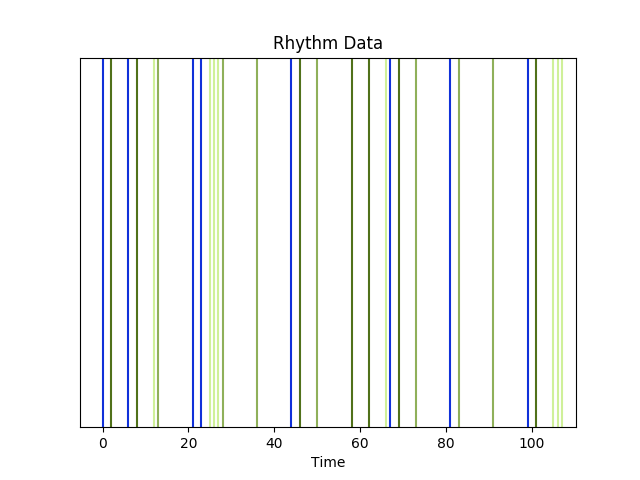
\includegraphics{figures/rhythm30.png}
    \caption{Rhythm Data}
    \label{fig:rhythm}
\end{figure}
\subsubsection{Hawkes}
The Hawkes dataset contains events generated by a Hawkes process. In a Hawkes process, event are generated as a point process, where the intensity associated with an event type is increased every time that the event occurs, and then decays over time to a base value. This is called a self-exciting process, and are descriptive of a process that tends to ``burst'', where an event signifies a likely reoccurrence of that event. A visualization of this type of sequence can be seen in Figure \ref{fig:Hawkes}.
\begin{figure}
    \centering
    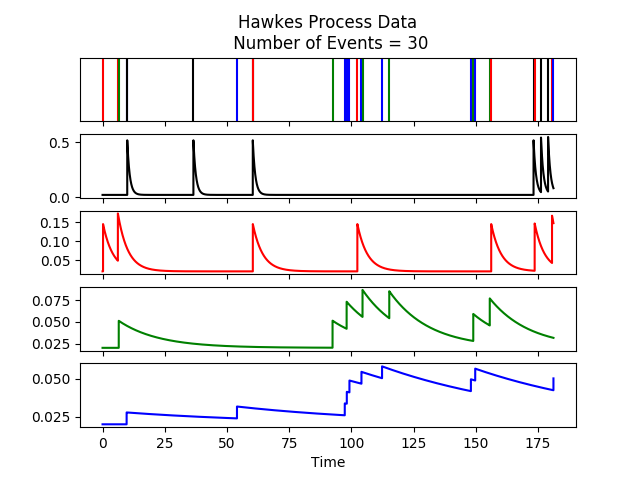
\includegraphics{figures/hawkes630.png}
    \caption{Hawkes Process Data}
    \label{fig:Hawkes}
    Hawkes Process event sequence and the  associated intensities for each event type
\end{figure}
\subsection{Natural Datasets}
\subsubsection{Github}
The Github dataset that we tested on was pulled from the Github BigQuery dataset, as announced at https://github.blog/2017-01-19-github-data-ready-for-you-to-explore-with-bigquery/ \cite{Github}. The dataset contains lists of commits to different repositories by users, and associated timestamps. For the purposes of the model, each repository was considered a sequence, and each commit was considered an event. The events were labelled by the user numerically, determined via order of appearance for the specific repository. We also restricted our dataset to only include sequences with at least two users that committed to it, and had at least 9 commits. There were approximately 1 million sequences in both the test and training set.

\subsubsection{Dota}
The Dota datasets are pulled from popular online game Dota 2. They contain chat logs between two teams of five during a match. The logs contain information regarding who is chatting, what is said, and when they are sent, as well as various metadata, including the label for which team won. The events were labelled by the anonymized label of the user associated. Notably, labels are always associated to the same team (i.e. 1-5 with team 1, 6-10 with team 2). Two data sets were developed, one for predicting the next users to chat (prediction), and another for predicting the outcome of the match (classification).

\subsubsection{Freecodecamp}
The Freecodecamp dataset contains anonymized data regarding learners' progress through online coding courses. Each student's progress was regarded as a sequence, and there were $\approx$ 60,000 students' data between the test and training sets with at least 9 events. Each completion of a module was considered an event, with about 450 different modules. Labelling of events was consistent for the same module across different sequences. Students were able to complete the same module multiple times, and modules were not necessarily completed in a specific order, although some tended to follow others. 
\subsubsection{Reddit}
There were two datasets we tested on from the popular online forum, Reddit. In the first dataset, an event sequence is associated to each user's posting history. For this dataset, events are labelled by which subreddit the user posts to. The second dataset associates an event sequence to a post. Each event in the sequence is a comment on the post, and is labelled by the user making the comment. 
\subsubsection{Quizlet}
The Quizlet dataset is the only example of the predicting correctness task in this paper. The Quizlet dataset involves anonymized data regarding students performance on vocabulary. Students performance on specific vocabulary words are tracked over time, and our network attempts to predict how likely a student is to correctly identify a vocabulary word.
\section{Experimental Procedure}
The process for comparing these two networks developed heavily over time. The network itself was developed primarily using the tools provided by the tensorflow package in Python3. Throughout the course, we consistently used 14 timescales for our hidden cells, which were originally set constants but were later dynamically calculated by the method describe in \ref{llmchap}. The learning rate was set to $10^{-3}$, and we used the Adam optimizer provided by tensorflow, as introduced in Kingma \& Ba, 2015 \cite{Adam}. \\\\Initially, we took care to experiment with a consistent number of hidden units, in the case of our experiments, assume that we used 100 hidden cells unless otherwise stated. Typically, the network only loaded the first 100 (or otherwise specified) events of a sequence for the prediction and predicting correctness tasks. This is to prevent the computer running on from running out of memory. We note at this point that all experiments were run on an Nvidia GeForce GTX 970, that caused hardware restrictions to the size of the network. The sequences associated with the classification task could not be truncated, as the entirety of the sequence might be essential to the class the sequence belongs to. For instance, consider a task where a sequence is classified solely on whether the network contains an event of a certain type. This classification cannot occur without full knowledge of the sequence. Prediction, however, makes a prediction at each timestep, and it is solely dependent on the events that occur before it. As a result, while a network might, and should, become better at predicting further into the sequence, the predictions up to the truncation are the same regardless of the following events. 
\\ \\When training on a specific dataset, we typically randomly drew 4000 sequences each for the training and test sets from the dataset, and then drew 10\% of the training set as a validation set. These random draws were done according to a seed such that the same datasets could be used for the LLM and LSTM testing. This was done due to the fact that typically only 10 trials were performed for a given set of parameters, so a single dataset draw that the network struggles to learn on wouldn't artificially make one of the networks seem to perform better (it is certainly still possible that some datasets are more likely to perform better under one network than the other in contrast to average, this can only be minimized by doing more trials). The pairing of trials with a random seed was implemented when we realized that there was a high variance in network performance, preventing any confidence in declaring one model better than the other for the dataset.
\\\\ The validation set that we create for each instance of the network is used for determining when the network has finished learning, and is beginning to overfit. It is also used when we select the best model from various hyperparameters. It is important to note here that there was a period of time during testing where an incompatibility between Python's random package and numpy package caused the validation and training sets to contain the same data. While this was later fixed, it did lead to some interesting revelations that we will address in \ref{ResSubSec}

\section{Results}
\subsection{Synthetic}
In our first stage of testing, we did many preliminary tests on different variations of the accumulator dataset. This enabled us to not only debug many aspects of the code we were running, it also provided a quick to test on outlet for determining any potential strengths and weaknesses of the LLM model. The initial results are displayed in Figures \ref{fig:SAres} and \ref{fig:SAresAUC}, with a 95\% confidence interval in a transparent color. It should be noted first that the graphs have been scaled to only show the top 10\% of the Accuracy and AUC metrics for this dataset in order to better display the differences in the networks.  It should be immediately apparent that the LLM underperforms on these datasets in comparison, as well as has a much larger confidence interval. In a naive sense, this might prevent us from declaring one network as better than the other with any confidence. However, when we pair up our trials of LLM and LSTM, we can consider the difference in metric (Accuracy or AUC) a random variable. We can then use these differences to test the hypothesis that the better performing network is, in fact, better. In this case we represent the difference as a t random variable, and calculate the associated p-value, which is represented at the bottom of our Figures. A value of $p<0.05$ represents a greater than 95\% confidence that the higher performing network is actually better suited to the task. In this case, the LSTM tends to perform better with high confidence. While it is not shocking that LSTM performs well, as it has historically been excellent at processing sequences, it is a bit disappointing that LLM underperforms. Nevertheless, it could certainly be the case that this task isn't ideal for the network. It is also possible that the structure of the LLM network is more likely to reach a local minimum that is far from the global. This would explain the high variance that the network experiences. 
\label{ResSubSec}
\begin{figure}
    \centering
    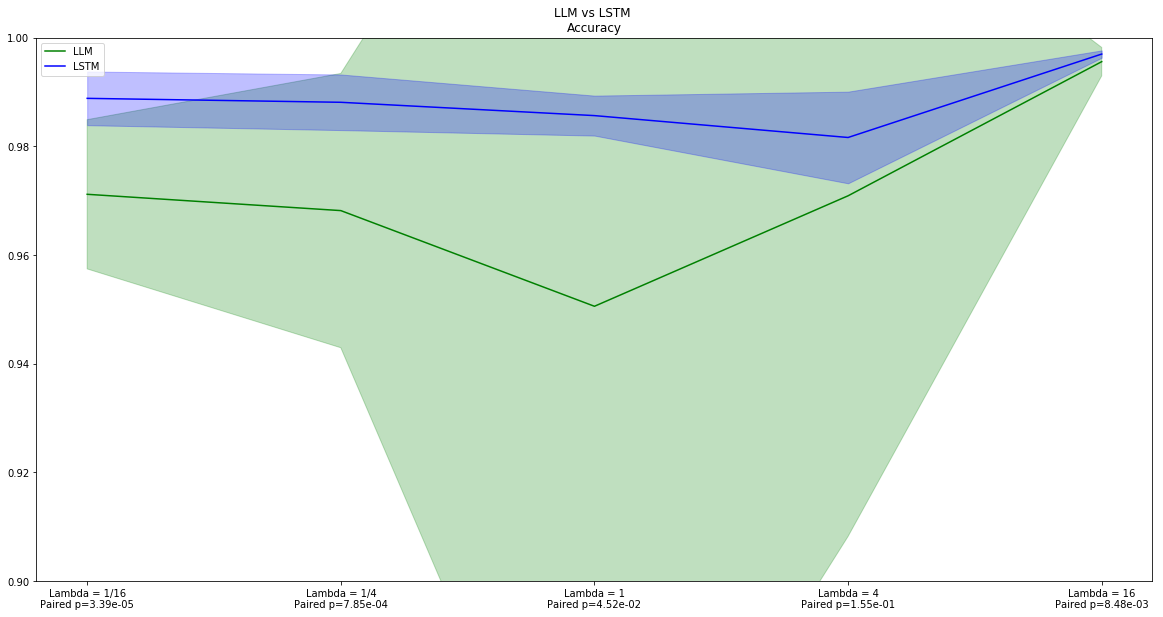
\includegraphics[width=1.0\textwidth]{figures/Synth_Accum_Data_Results.png}
    \caption{Accuracy of Network on Different Decay Rates}
    \label{fig:SAres}
    Accuracy Results for LLM (Green) and LSTM (Blue) for different Accumulator Decay Rates
\end{figure}
\begin{figure}
    \centering
    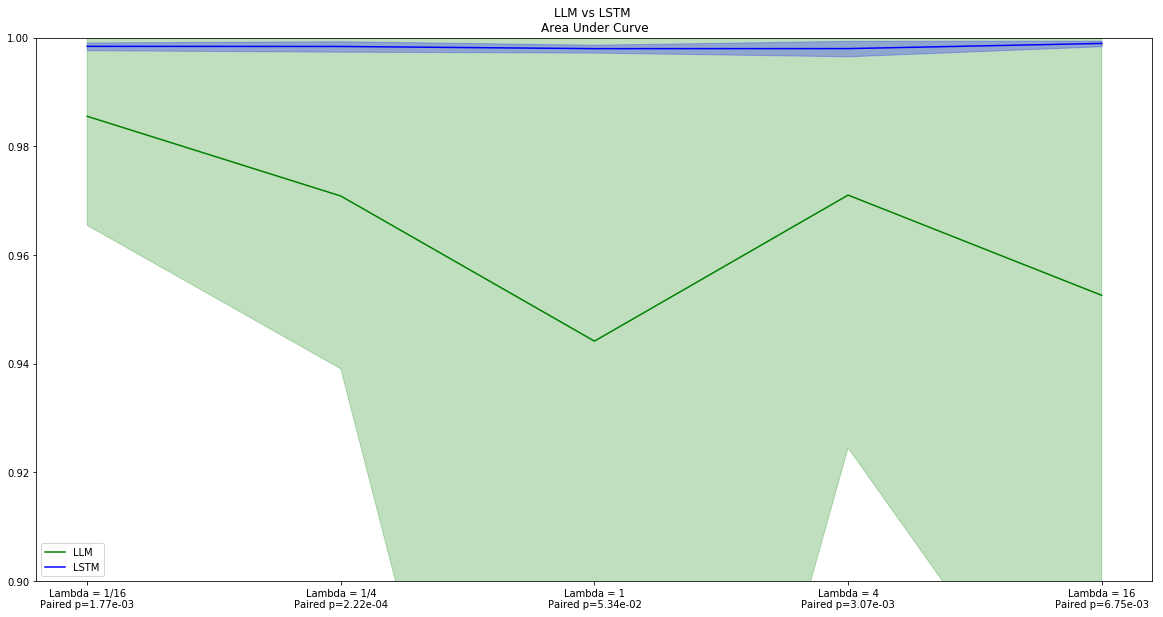
\includegraphics[width=1.0\textwidth]{figures/Synth_Accum_Data_Results_AUC.png}
    \caption{Area Under Curve of Network on Natural Datasets}
    \label{fig:SAresAUC}
    AUC Results for LLM (Green) and LSTM (Blue) w for different Accumulator Decay Rates
\end{figure}
\\\\For the accumulator dataset, we next looked into predicting the next event that would occur in an accumulator sequence. This should be a simple task if the network is able to recognize the structure of the sequence as two Poisson processes. This is due to the fact that Poisson processes are memoryless, so at any point in time, the predictor should simply predict the sequence with a shorter timescale, which is most likely to be the most common event up to that point. We ran several trials on this task, and present the results in Figure \ref{fig:pred_acc}.
\begin{figure}
    \centering
    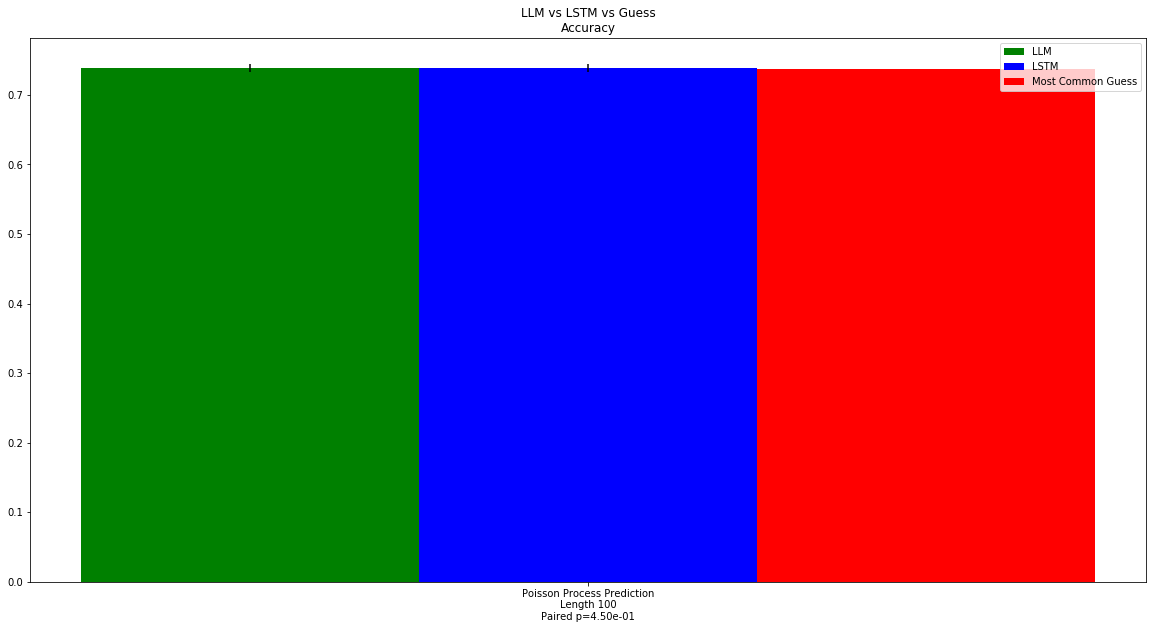
\includegraphics[width=1.0\textwidth]{figures/Accum_Pred.png}
    \caption{Accuracy of Network Predicting Poisson Processes}
    \label{fig:pred_acc}
    
\end{figure}
\\\\ It seems that this task is simple enough that both of the networks are able to learn this ideal predictor.
\\\\  Next we looked into the rhythm dataset. We first ran experiments on the classification task described in \ref{sec:rhythm}. We restricted the length of the sequences to 10, 30, and 100 for different trials to explore how more information affected the networks' ability to classify. Hypothetically, an ideal classifier would classify the sequence as a 1 up until an anomaly is detected. The generation process does leave the possibility of an ``anomalous" sequence not registering as such. This is due to the fact that an event with an altered lag time not appearing in the sequence. Regardless, we present the results of our experiment in Figures \ref{fig:rhy_acc} and \ref{fig:rhy_auc}.
\begin{figure}
    \centering
    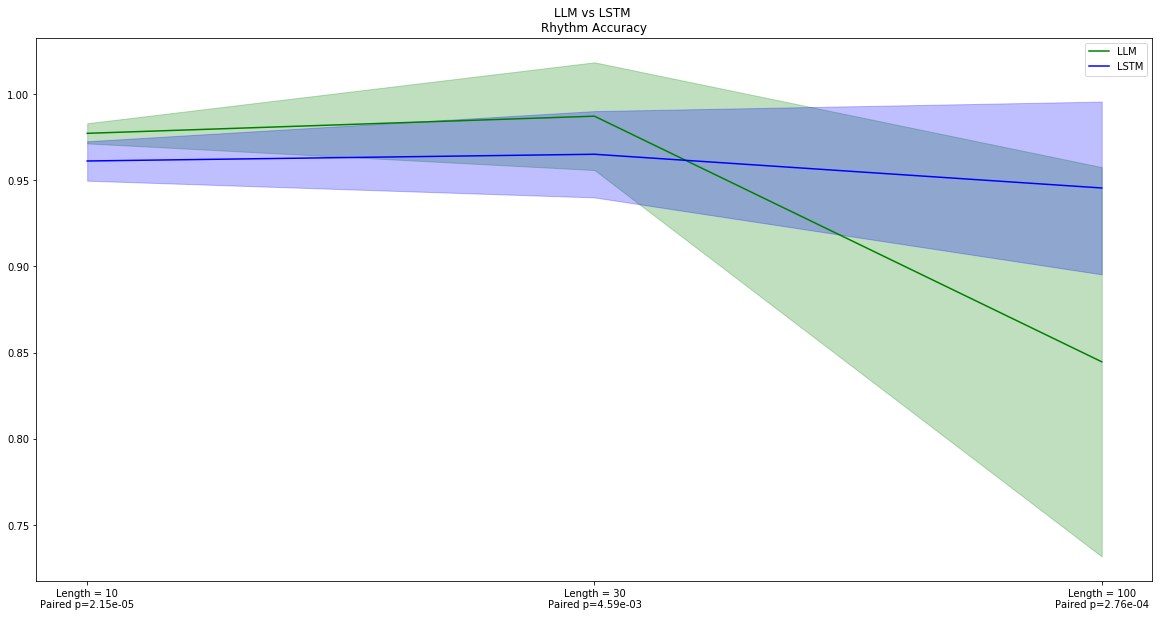
\includegraphics[width=1.0\textwidth]{figures/Rhythm_Accuracy.png}
    \caption{Accuracy of Network on Rhythm Dataset}
    \label{fig:rhy_acc}
    Accuracy Results for LLM (Green) and LSTM (Blue) with different sequence lengths
\end{figure}
\begin{figure}
    \centering
    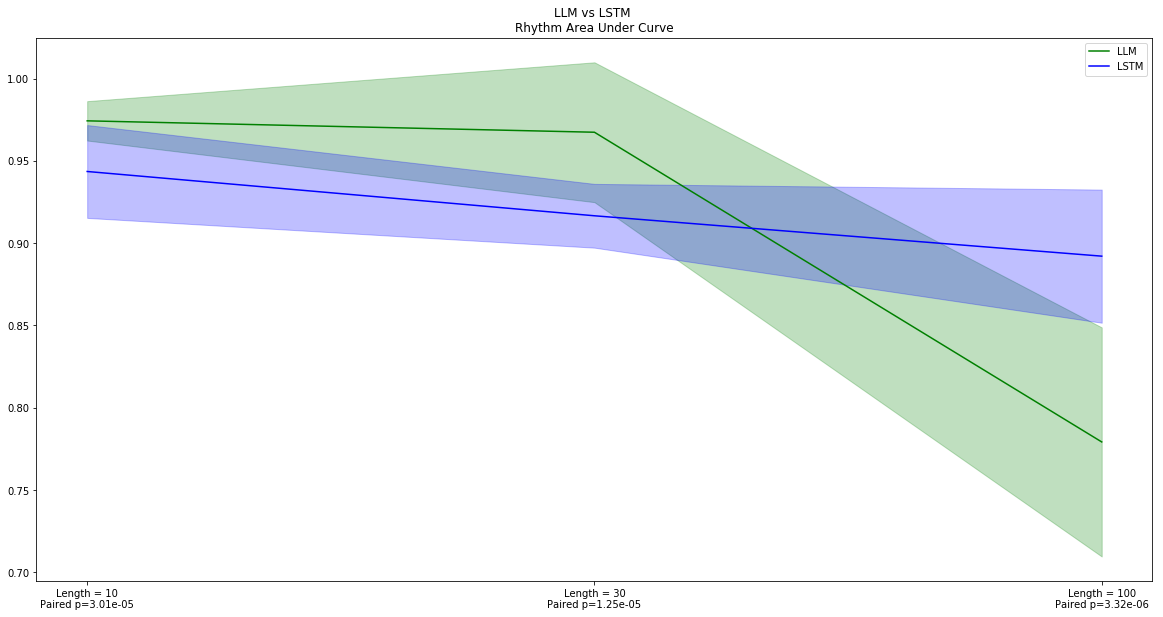
\includegraphics[width=1.0\textwidth]{figures/Rhythm_AUC.png}
    \caption{Area Under Curve of Network on Rhythm Datasets}
    \label{fig:rhy_auc}
    AUC Results for LLM (Green) and LSTM (Blue) with different sequence lengths
\end{figure}
Interestingly the LLM performs significantly better for the shorter sequences, but there is a drop in performance on the longer sequence. This shouldn't happen, when a longer sequence should only provide a greater ability to classify. In this case, one must assume that the network is either forgetting its classification (the presence of an anomaly), or it is retaining too much information, and is overwhelmed by too much memory in this case, not able to forget quickly enough. We ran another test on the data, this time with a wider net of timescales, in order to test whether the latter could be true.
\begin{figure}
    \centering
    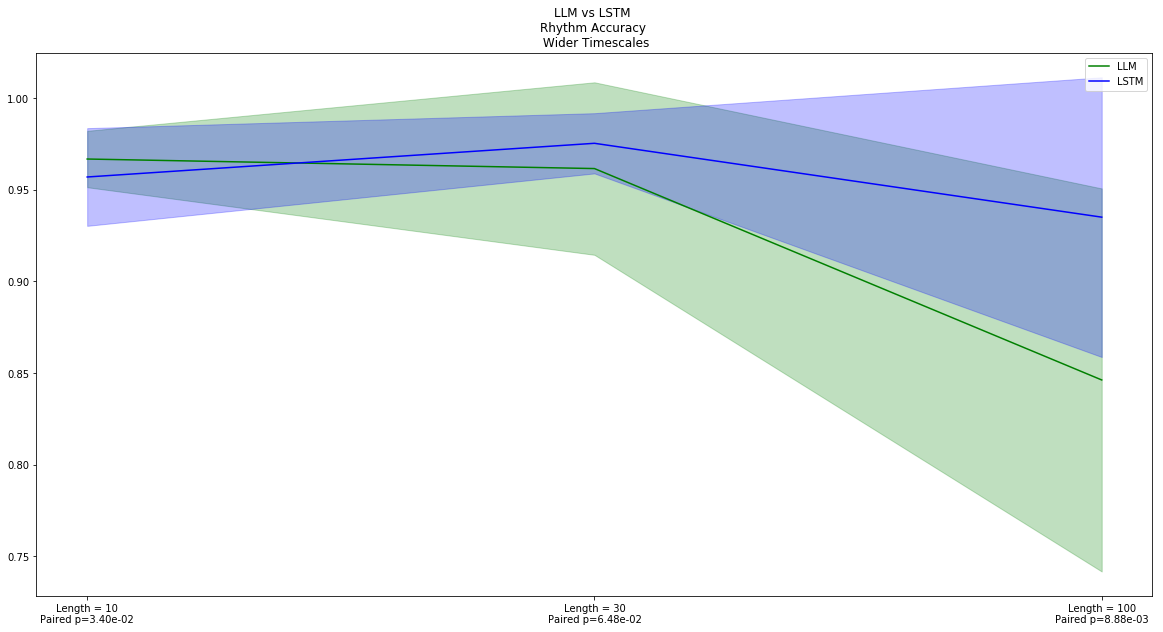
\includegraphics[width=1.0\textwidth]{figures/Rhythm_Wide_Accuracy.png}
    \caption{Accuracy of Network on Rhythm Dataset with larger timescale range}
    \label{fig:RhyWide}
\end{figure}
\textit{ }\\\\Figure \ref{fig:RhyWide} shows the results from this experiment. It is apparent that there is something else going on causing the drop in performance, and would warrant further investigation in later work. Despite this, on sequences that both networks did ``well'' on, the LLM performed better at this classification task. 
\\\\ Finally, we tested on our last dataset, the Hawkes dataset. For this dataset, the networks should be attempting to mimic the intensity functions of the various Hawkes processes. The process with the highest intensity at a given time step should be the most likely event to occur. Using this, we built out an estimator for the average performance of a predictor.
\begin{figure}
    \centering
    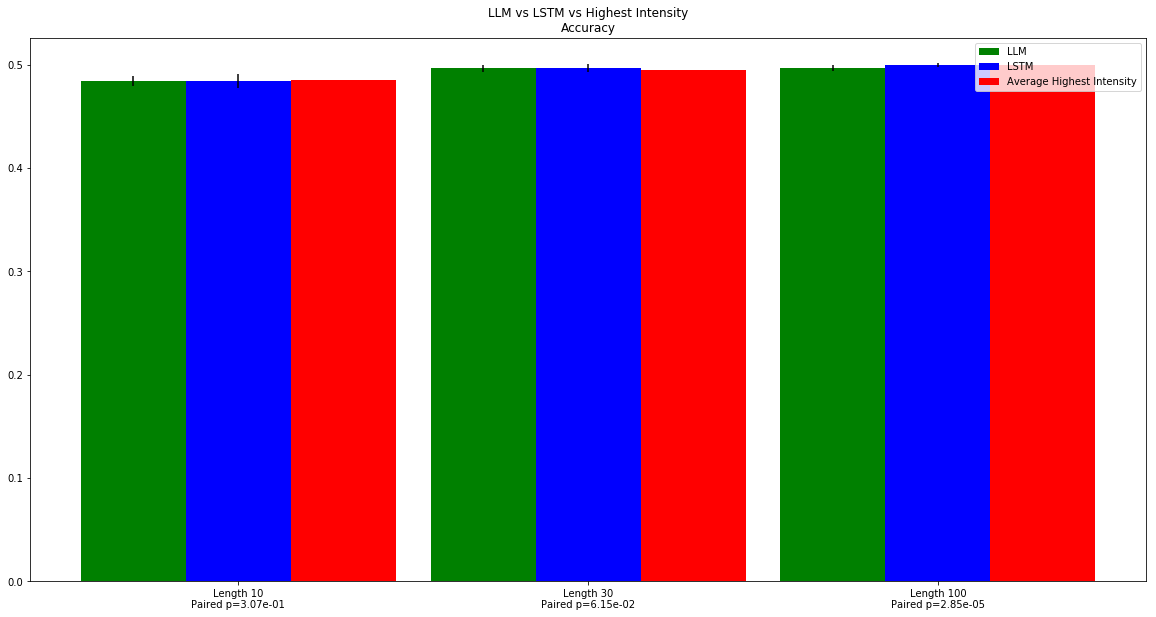
\includegraphics[width=1.0\textwidth]{figures/Hawkes1.png}
    \caption{Accuracy of Network on Hawkes Prediction}
    \label{fig:hawkes1}
    Accuracy results for LLM (Green) and LSTM (Blue) with 100 hidden units compared to the ideal predictor.
\end{figure}
\\\\Figure \ref{fig:hawkes1} shows the accuracy both networks achieve on the Hawkes dataset. We also present how a predictor would fare if it had knowledge of the intensity functions of each event type. 
\subsection{Natural}

The natural datasets were first experimented on with a consistent number of hidden units (100). In Figures \ref{fig:res} and \ref{fig:resAUC} , we display the accuracy results and AUC results over several of the datasets. 
\begin{figure}
    \centering
    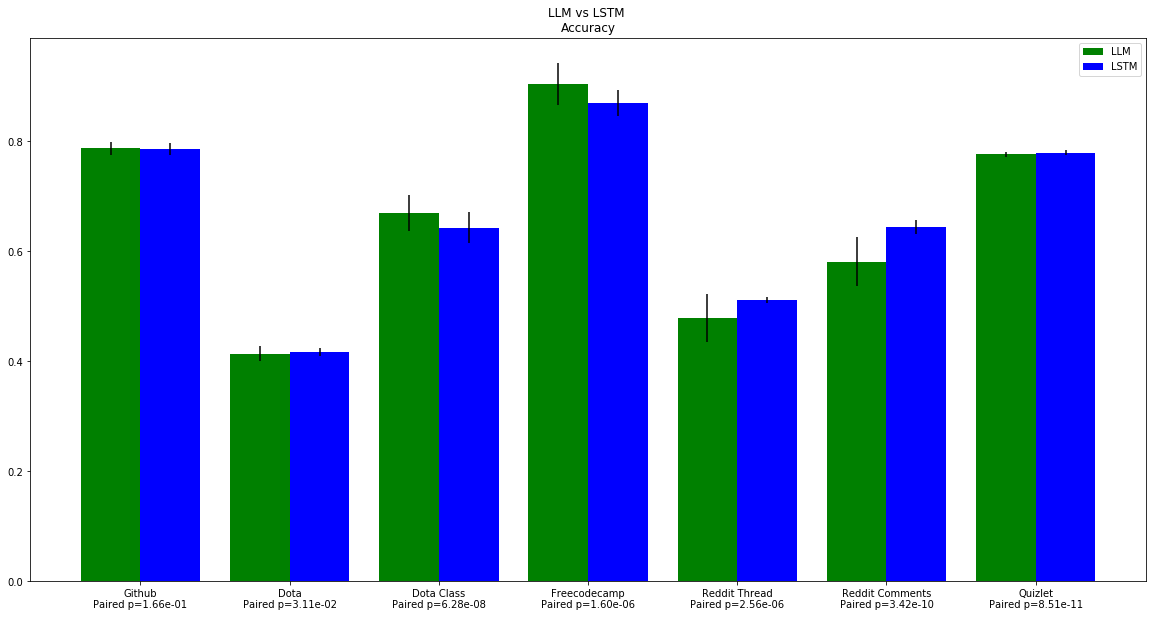
\includegraphics[width=1.0\textwidth]{figures/Data_Results.png}
    \caption{Accuracy of Network on Natural Datasets}
    \label{fig:res}
    Accuracy Results for LLM (Green) and LSTM (Blue) with 100 hidden units
\end{figure}
\begin{figure}
    \centering
    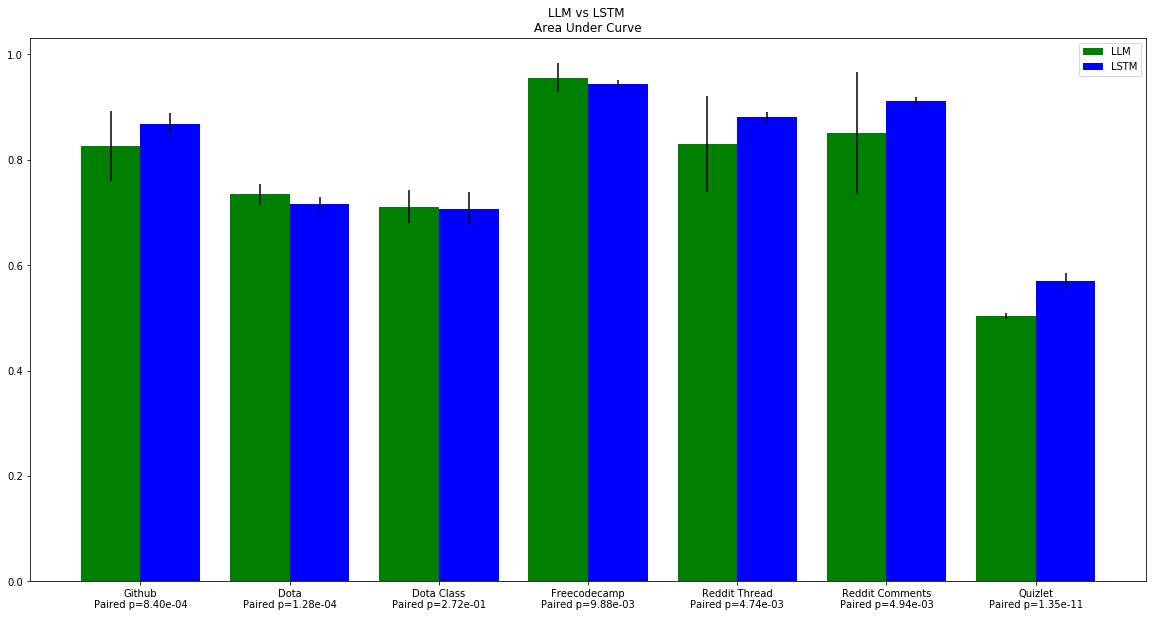
\includegraphics[width=1.0\textwidth]{figures/Data_Results_AUC.png}
    \caption{Area Under Curve of Network on Natural Datasets}
    \label{fig:resAUC}
    AUC Results for LLM (Green) and LSTM (Blue) with 100 hidden units
\end{figure}
\\\\The error bars displayed are 95\% confidence intervals on the performance of the network. Once again, they are frequently to large to confidently declare one network as performing better. In the figures, we list the p-value of the hypothesis that the better performing network is better suited for the task under the given metric. There does seem to be a few tasks that LLM outperforms LSTM, as well as tasks that LSTM is better on. But, for a given network with set parameters, even if the networks have the same number of cells, they do not necessarily have the same number of weights to learn. We have the number of trainable weights that there are in each network for different numbers of hidden cells can be seen in Table \ref{tab:hiddenweights}.
  




\begin{table}
    \caption[Number of Weights]{Table noting the number of weights associated with each network and different numbers of hidden cells.}
    \label{tab:hiddenweights}
    \begin{center}
    \vspace{-4cm}
	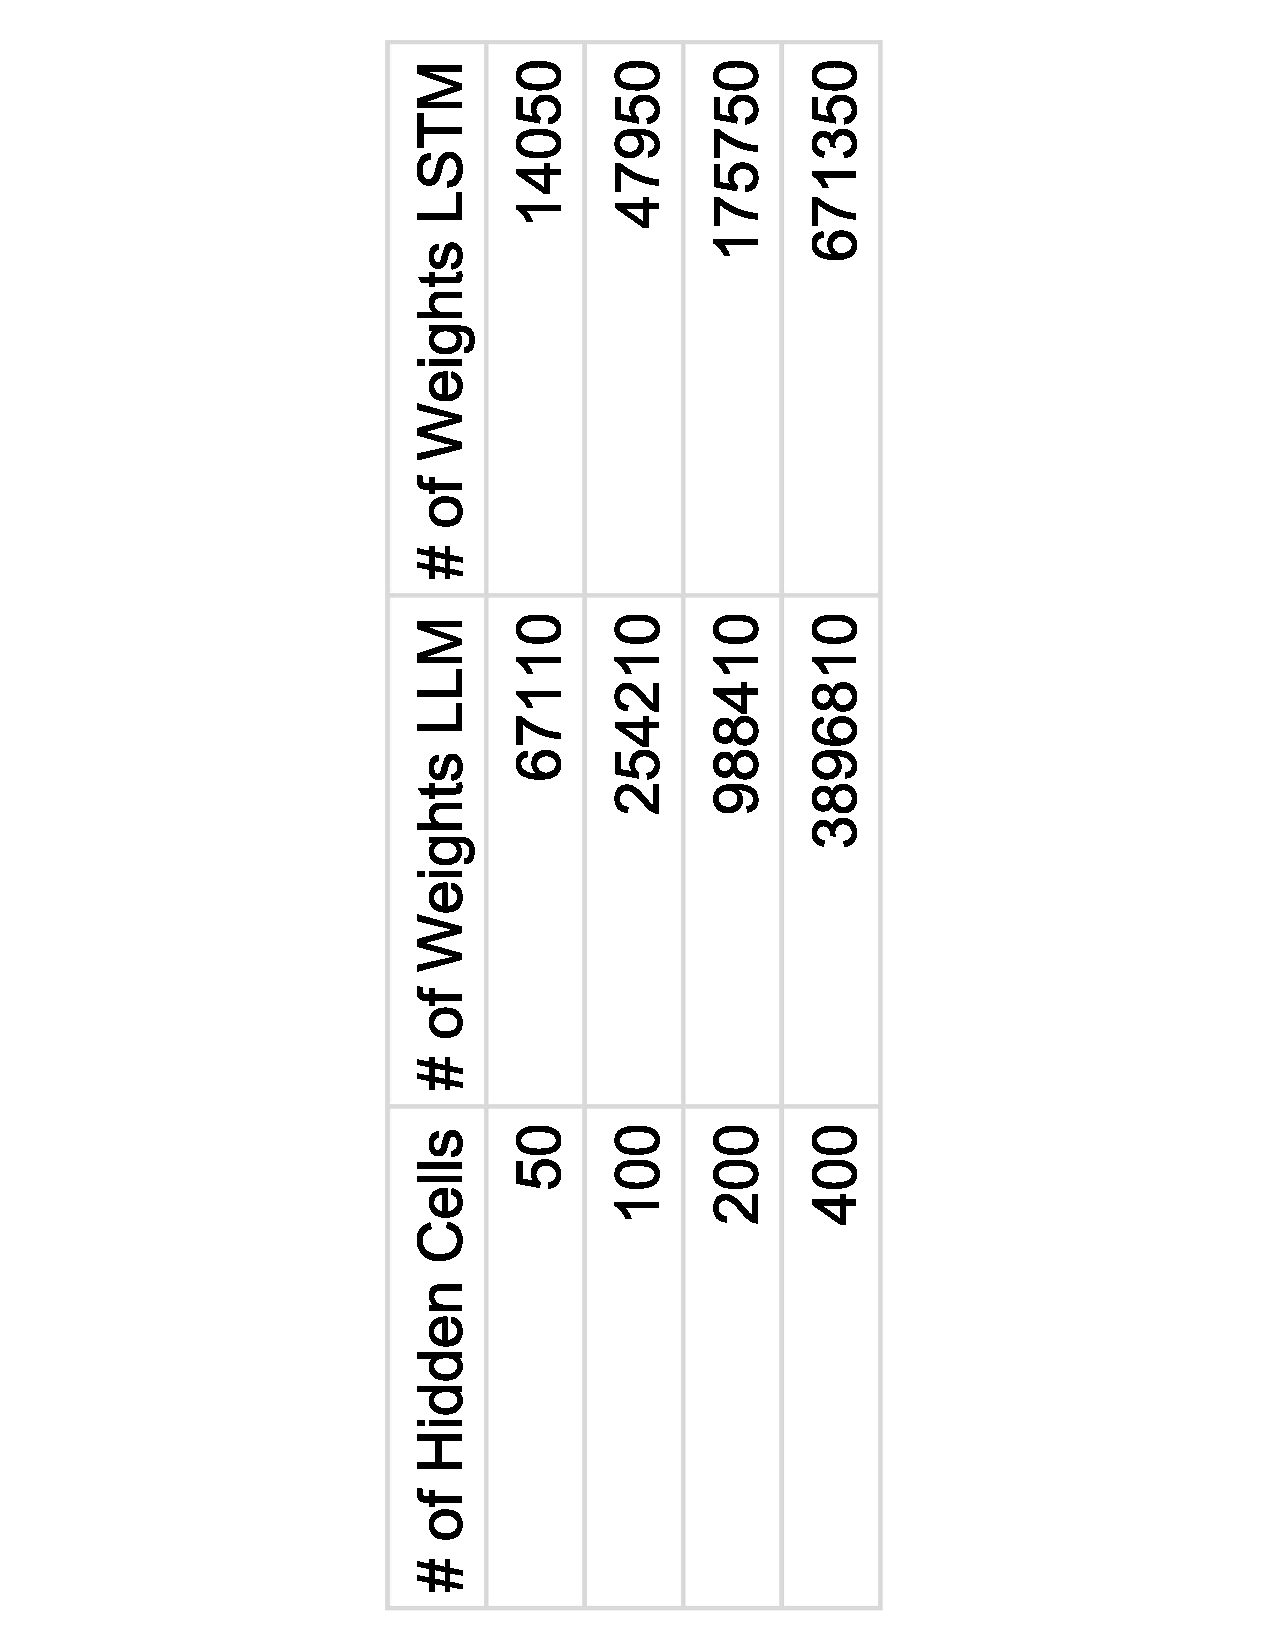
\includegraphics[width=5in, angle=270]{figures/Hidden_Weights.pdf}
    \end{center}
\end{table}
\textit{ }
\\Even if there were the same number of weights to learn, that might not be ideal for the network. We combat this by introducing a hypertuning of the parameters. We train the networks with several different numbers of hidden cells. We then use the accuracy on the validation set to determine which network size is ideal for the task. We use the validation set since it is used to determine when the model has fully trained. We then reran the paired tests with the optimal hyperparameters to calculate a new p value.
\begin{figure}
    \centering
    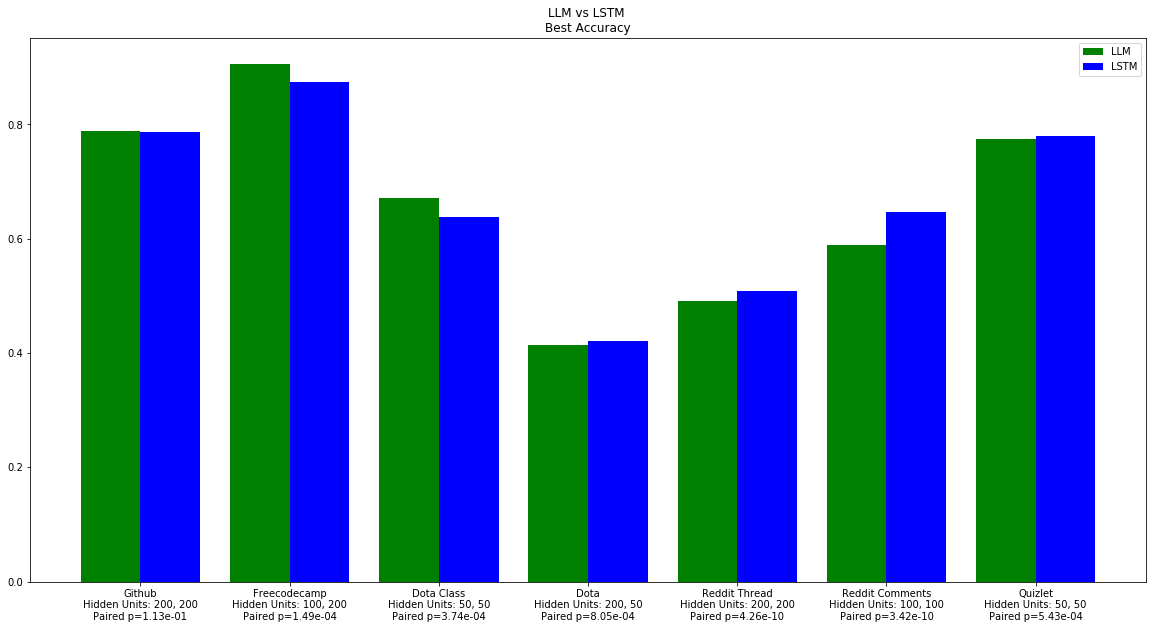
\includegraphics[width=1.0\textwidth]{figures/Data_Results_Best.png}
    \caption{Best Accuracy of Network on Natural Datasets}
    \label{fig:resBest}
    Accuracy Results for LLM (Green) and LSTM (Blue) with hypertuned hidden units
\end{figure}
\\\\
There is one interesting result that we found due to an error in generating the validation set. For a while, there was an artificial correlation between the training and validation sets that didn't exist with the test set. This caused the networks to naturally overtrain until the training sets loss was at a minima. What may seem surprising, is the contrast between LLM and LSTM in terms of difference in performance. In Figures \ref{fig:llmValid} and \ref{fig:lstmValid} we compare the performance on accuracy with and without validation halting on several of the datasets.
\begin{figure}
    \centering
    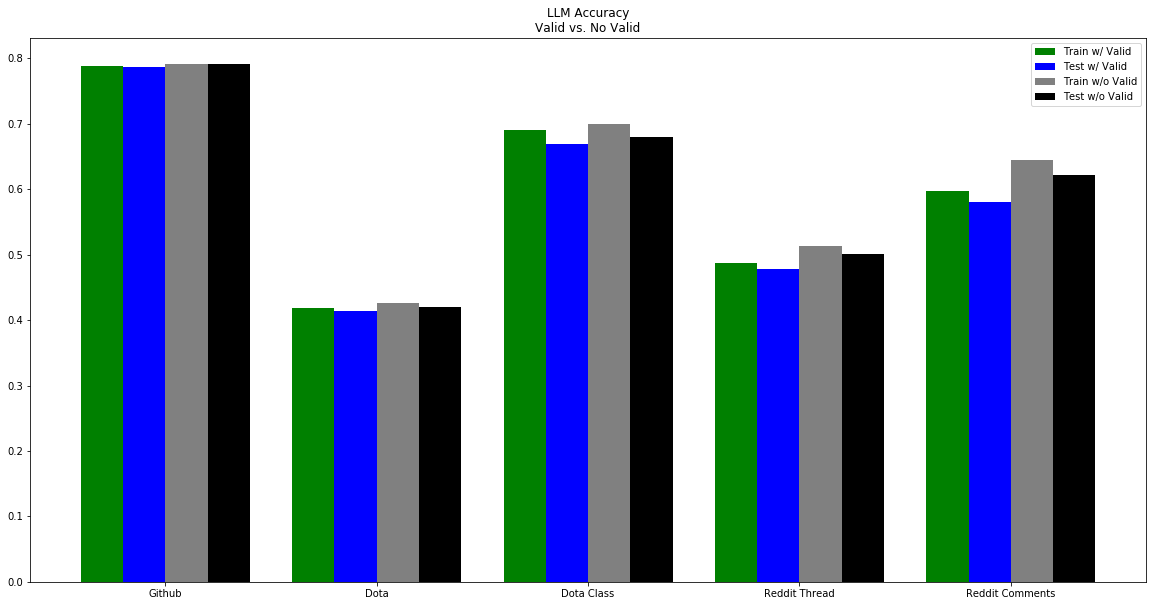
\includegraphics[width=1.0\textwidth]{figures/LLM_Valid.png}
    \caption{Accuracy of LLM comparing Validation}
    \label{fig:llmValid}
\end{figure}

\begin{figure}
    \centering
    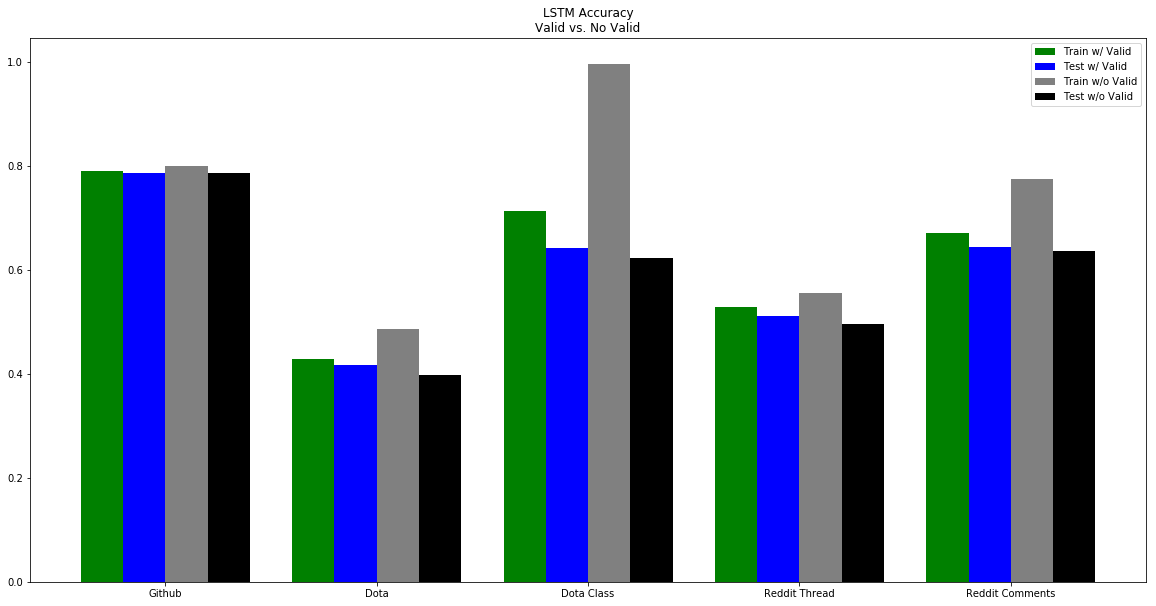
\includegraphics[width=1.0\textwidth]{figures/LSTM_Valid.png}
    \caption{Accuracy of LSTM comparing Validation}
    \label{fig:lstmValid}
\end{figure}
\textit{ }\\What should be immediately apparent is that the LSTM overfits to the training set (in some cases much more noticeably than others). This occurs at the detriment of the testing accuracy. Meanwhile, the LLM faces no penalty for the lack of validation. In fact, it appears that it even receives a slight boost to both the training and testing accuracy. 
\\\\ It makes sense that the LLM would be less prone to overfit, since it imposes a structure to the time data and ability to forget that the LSTM does not have. It naturally imposes regularization. We also take the fact that LLM performs similarly with and without validation as evidence that the memory of the sequence does in fact mirror the memory of the network. 
\subsubsection{Discussion of Results}
Before we begin a full discussion of our results, we present Table \ref{tab:naive} denoting the accuracy of three naive prediction tactics. First we examine simply guessing the previous event. Next, we try guessing the most common event in the sequence. Finally, we guess that the next event will be the sequentially next event, i.e. if an event was initially follow by an event previously, predict that it will happen again. It is important to note here that the only predictions we posit for the classification and predicting correctness tasks, we only put forward the most common classification or binary label as the naive approach.\\
\begin{table}
    \caption[Naive Predictions]{Table describing the accuracy of various naive approaches}
    \label{tab:naive}
    \begin{center}
	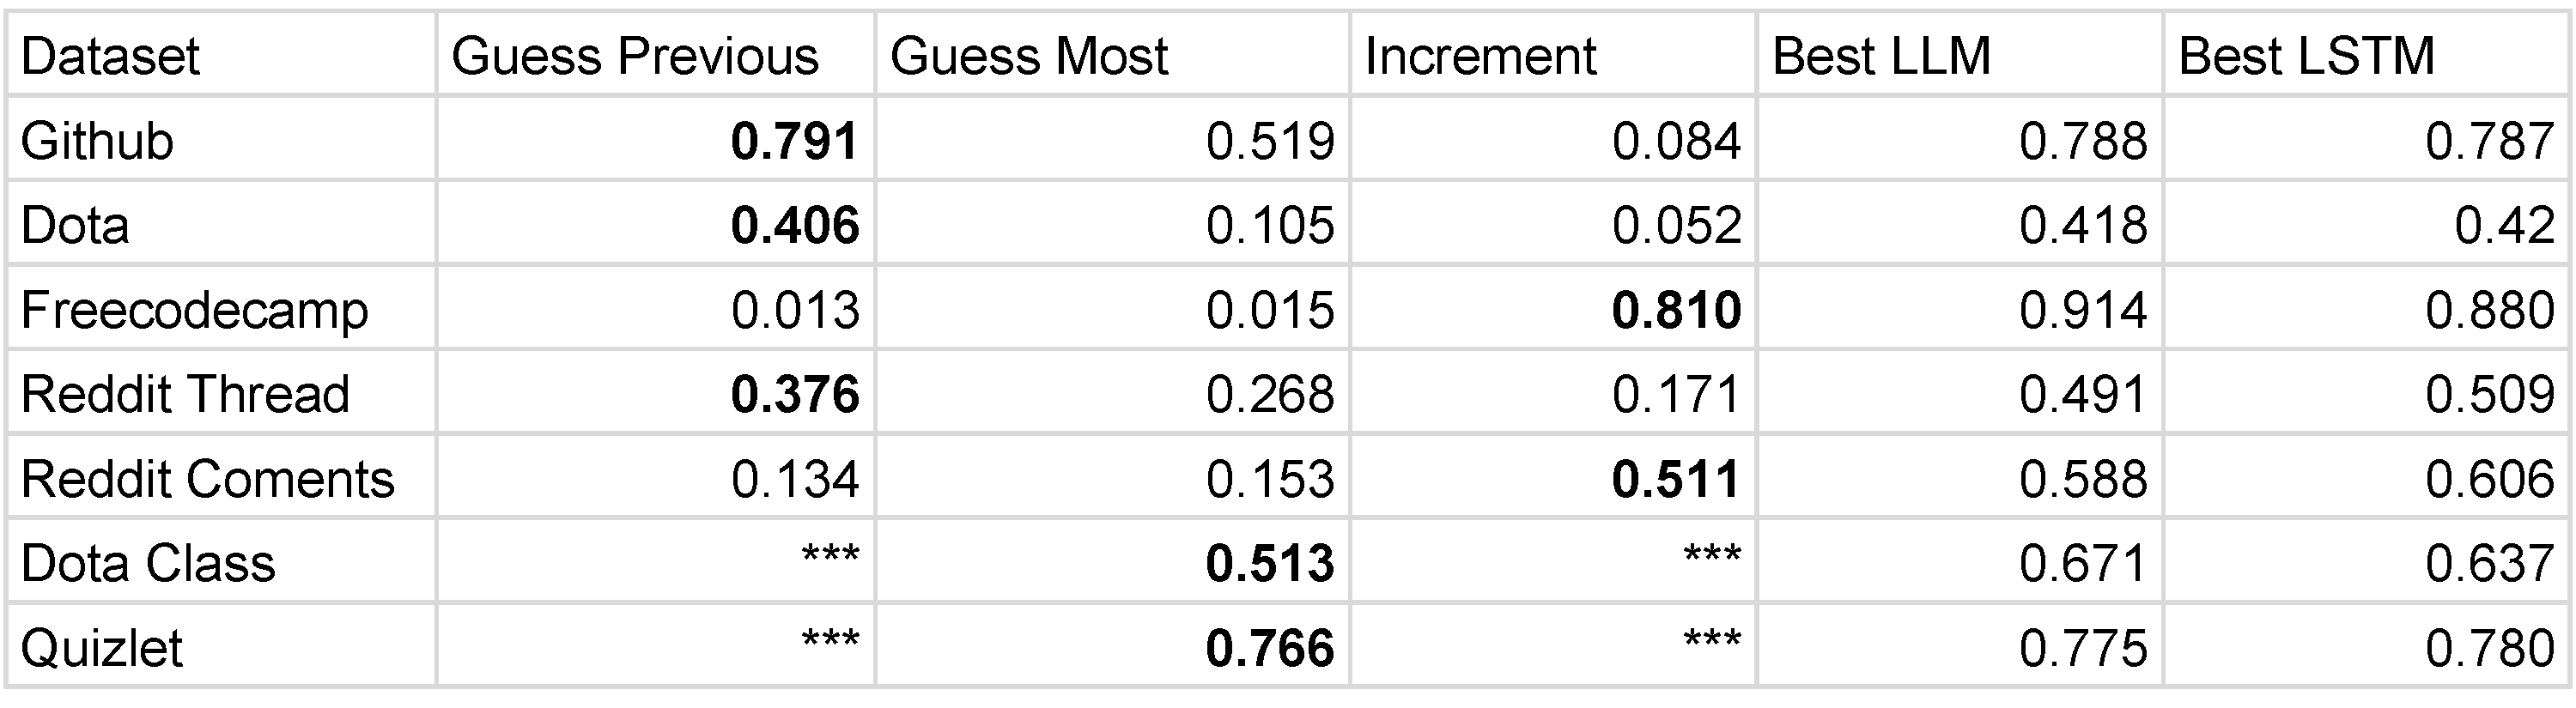
\includegraphics[width=\textwidth]{figures/Naive_Predicts.pdf}
    \end{center}
\end{table}
\\ Given these tables, we can conclude that neither network learned anything meaningful about the Github, Dota, or Quizlet datasets. Both the LLM and LSTM failed to learn anything about these datasets beyond naive statistics (less than a total difference of 5\% in accuracy). Interestingly, these datasets were the ones that the networks performed most similarly on (less than a total difference of 1\% in accuracy from each other). Meanwhile, the LLM performed better on the classification dataset, as well as the Freecodecamp dataset. Interestingly, these were two of the three datasets in our tests that had consistently labelled events across sequence, versus the reddit datasets, which had subreddits labelled in order.
%\\\\This didn't seem to be the case, however, in our synthetic datasets. These typically featured consistently labelled event types, and yet
\\\\ We once again feel that it is important to note the implications of Figures \ref{fig:llmValid} and \ref{fig:lstmValid}. The ability of LLM to self regularize seems to be indicative of a greater structure to the data. The LSTM is able to mimic the structure, but when given the opportunity to overfit to the training data, it seems to do so at the expense of the testing set. 